\pdfoutput=1
\documentclass[12pt]{article}

\usepackage[toc,page]{appendix}

\usepackage[utf8]{inputenc}

\usepackage{amsthm}
\usepackage{longtable}

\newtheorem{theorem}{Theorem}
\newtheorem{lemma}[theorem]{Lemma}
\theoremstyle{definition}
\newtheorem*{definition}{Definition}

\usepackage{tikz}
\usetikzlibrary{calc}

\usepackage{enumerate}
\usepackage{enumitem}

\usepackage{etoolbox}
\AtBeginEnvironment{quote}{\small}

\usepackage{mathtools}
\DeclarePairedDelimiter{\floor}{\lfloor}{\rfloor}

\usepackage[colorlinks=true,urlcolor=blue,linkcolor=blue]{hyperref}

\begin{document}

\title{CASPaxos: Replicated State Machines without logs}

\author{Denis Rystsov\\\texttt{rystsov.denis@gmail.com}}

\maketitle

\begin{abstract}
CASPaxos is a replicated state machine (RSM) protocol, an extension of Synod (Single Decree Paxos). Unlike Raft and Multi-Paxos, it doesn't use leader election and log replication, so it avoids associated complexity. Its symmetric peer-to-peer approach achieves optimal commit latency in the wide-area network and doesn't cause cluster unavailability when any $\floor{N/2}$ of $N$ nodes crash.

The lightweight nature of CASPaxos allows new combinations of RSMs in the designs of distributed systems. For example, a representation of a key/value storage as a hashtable with independent RSM per key increases fault tolerance and improves performance on multi-core systems compared with a hashtable behind a single RSM.

This paper describes CASPaxos protocol, formally proves its safety properties, covers cluster membership change and evaluates the benefits of a CASPaxos-based key/value storage.
\end{abstract}

\section{Introduction}

Multi-Paxos\cite{lamport01} and Raft\cite{raft} protocols allow a collection of machines to work as a single state machine tolerating failures and network issues. The protocols guarantee safety in the presence of arbitrary node crashes, message loss and reordering; and preserve liveness when at most $\floor{N/2}$ of $N$ machines are down or disconnected.

The problem of keeping a RSM work when its nodes crash and network is partitioned is isomorphic to the problem of master-master replication of a linearizable distributed storage under the same conditions. So those protocols are widely used in the industry as a foundation of such databases as Chubby\cite{chubby}, Etcd\footnote{\href{https://github.com/coreos/etcd}{https://github.com/coreos/etcd}}, Spanner\cite{spanner}, etc.

Despite the wide adoption, there are a lot of indications that the protocols are complex. Diego Ongaro and John Ousterhout write in "In Search of an Understandable Consensus Algorithm"\cite{raft}:

\begin{quote}
In an informal survey of attendees at NSDI 2012, we found few people who were comfortable with Paxos, even among seasoned researchers. We struggled with Paxos ourselves; we were not able to understand the complete protocol until after reading several simplified explanations and designing our own alternative protocol, a process that took almost a year
\end{quote}

Google's engineers write about their experience of building a Paxos-based database in the "Paxos Made Live"\cite{chubby} paper:

\begin{quote}
Despite the existing literature in the field, building such a database proved to be non-trivial \ldots{} While Paxos can be described with a page of pseudo-code, our complete implementation contains several thousand lines of C++ code \ldots{} There are significant gaps between the description of the Paxos algorithm and the needs of a real-world system.
\end{quote}

The complexity of the RSM protocols may explain the bugs in the replication layer of the established databases. Kyle Kingsbury made a comprehensive research\footnote{\href{https://aphyr.com/tags/jepsen}{https://aphyr.com/tags/jepsen}} of the distributed consistent storages and found violations of linearizability in some version of almost every system he tested including MongoDB, Etcd, Consul, RethinkDB, VoltDB and CockroachDB.

Besides complexity, those protocols have temporary availability problems when a leader crashes or is isolated. The "There Is More Consensus in Egalitarian Parliaments" paper\cite{epaxos} describes the negative implications of a leader-based system which are applicable both to Multi-Paxos and Raft:

\begin{quote}
Traditional Paxos variants are sensitive to both long-term and transient load spikes and network delays that increase latency at the master \ldots{} this single-master optimization can harm availability: if the master fails, the system cannot service requests until a new master is elected \ldots{} Multi-Paxos has high latency because the local replica must forward all commands to the stable leader.
\end{quote}

{\bf Contributions.} I present CASPaxos, a novel protocol for building RSM that avoids complexity and pitfalls of the log-based systems.

Multi-Paxos based system is a RSM built on top of a replicated log which treats every log entry as a command. The replicated log is modelled as an array of Synod instances. According to Raft paper, its complexity comes from the composition rules:

\begin{quote}
We hypothesize that Paxos’ opaqueness derives from its choice of the single-decree subset as its foundation \ldots{} The composition rules for Multi-Paxos add significant additional complexity and subtlety.

One reason is that there is no widely agreed upon algorithm for multi-Paxos. Lamport’s descriptions are mostly about single-decree Paxos; he sketched possible approaches to multi-Paxos, but many details are missing. As a result, practical systems bear little resemblance to Paxos. Each implementation begins with Paxos, discovers the difficulties in implementing it, and then develops a significantly different architecture \ldots{} real implementations are so different from Paxos that the proofs have little value
\end{quote}

Instead of using Synod as a building block CASPaxos extends it, so there is no composition and the associated complexity.

According to an experimental study\cite{raft} and the number of open source implementations\footnote{\href{https://raft.github.io/\#implementations}{https://raft.github.io/\#implementations}} Raft succeeded in its goal to be understandable. However, its complexity is still comparable with Multi-Paxos: both systems\cite{chubby}\cite{raft} have several thousand of lines of code, both use concepts of leader election and leases, both are based on logs and require log compaction. CASPaxos is significantly simpler: it doesn't have those pieces and its implementation\footnote{\href{https://github.com/gryadka/js}{https://github.com/gryadka/js}} is less than 500 lines of code.

Being just an extension of Synod, CASPaxos uses its symmetric peer-to-peer approach and automatically achieves the goals set in the EPaxos\cite{epaxos} paper: (1) optimal commit latency in the wide-area when tolerating one and two failures, under realistic conditions; (2) uniform load balancing across all replicas (thus achieving high throughput); and (3) graceful performance degradation when replicas are slow or crash.

{\bf Verification}. The formal proof is included into the appendix \ref{appendix:proof}, Tobias Schottdorf\footnote{\href{https://tschottdorf.github.io/single-decree-paxos-tla-compare-and-swap}{https://tschottdorf.github.io/single-decree-paxos-tla-compare-and-swap}} and Greg Rogers\footnote{\href{https://medium.com/@grogepodge/tla-specification-for-gryadka-c80cd625944e}{https://medium.com/@grogepodge/tla-specification-for-gryadka-c80cd625944e}} independently model checked the protocol with TLA+, and the implementation was successfully tested with faults injection methodology.

\section{Algorithm}

We begin by briefly describing the Synod protocol from the perspective of master-master replication, followed by a step by step comparison with CASPaxos.

\subsection{Synod}

An implementation of the Synod protocol is an initializable only once distributed register. When several clients try to initialize it concurrently, the requests either prevent each other from continuing, or a single initialization succeeds. Once a client receives a confirmation, all the follow-up initializations must return the already chosen value.

The register belongs to the CP category of the CAP theorem, so it gives up availability when more than $\floor{N/2}$ nodes are down but always preserves consistency (safety, linearizability).

The system has three roles.

\begin{description}[align=left]
  \item [Clients] initiate a request by communicating with a proposer; clients may be stateless, the system may have arbitrary numbers of clients.
  \item [Proposers] perform the initialization by communicating with acceptors. Proposers keep minimal state needed to generate unique increasing update IDs (ballot numbers), the system may have arbitrary numbers of proposers.
  \item [Acceptors] store the accepted value, the system should have $2F+1$ acceptors to tolerate $F$ failures.
\end{description}

\begin{figure}[!h]
  \centering
  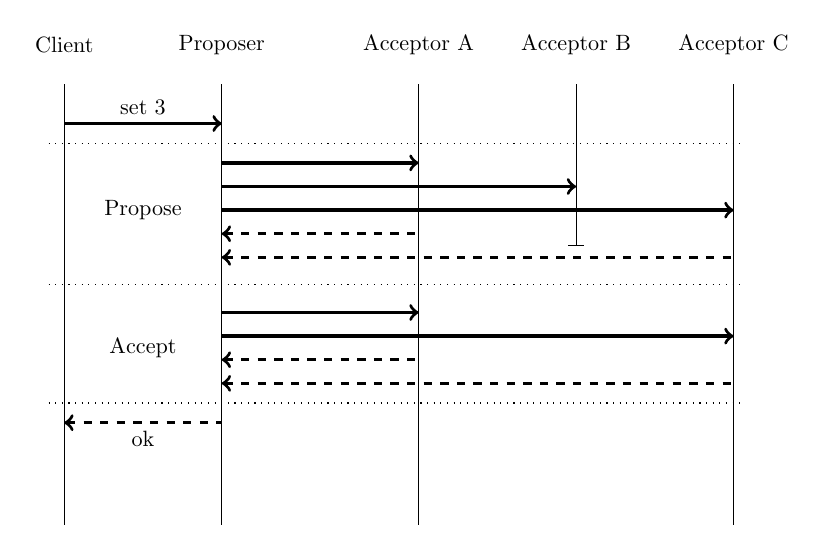
\begin{tikzpicture}[y=-1cm]
    \node at (0,-0.5)[scale=0.8]{Client};
    \node at (2,-0.5)[scale=0.8]{Proposer};
    \node at (4.5,-0.5)[scale=0.8]{Acceptor A};
    \node at (6.5,-0.5)[scale=0.8]{Acceptor B};
    \node at (8.5,-0.5)[scale=0.8]{Acceptor C};
    
    \draw (0,0) -- (0,5.6);
    \draw (2,0) -- (2,5.6);
    \draw (4.5,0) -- (4.5,5.6);
    \draw (6.5,0) -- (6.5,2.05);
    \draw (8.5,0) -- (8.5,5.6);
    \draw (6.4,2.05) -- (6.6,2.05);
  
    \draw[dotted] (-0.2,0.75) -- (8.6,0.75);
    \draw[dotted] (-0.2,2.55) -- (8.6,2.55);
    \draw[dotted] (-0.2,4.05) -- (8.6,4.05);
  
    \begin{scope}[very thick]
      \draw[->] (0,0.5) -- (2,0.5) node[above, midway, scale=0.8]{set 3};
      
      \node at (1,1.6)[scale=0.8]{Propose};
      \draw[->] (2,1) -- (4.5,1);
      \draw[->] (2,1.3) -- (6.5,1.3);
      \draw[->] (2,1.6) -- (8.5,1.6);
      \draw[<-, dashed] (2,1.9) -- (4.5,1.9);
      \draw[<-, dashed] (2,2.2) -- (8.5,2.2);
  
      \node at (1,3.35)[scale=0.8]{Accept};
      \draw[->] (2,2.9) -- (4.5,2.9);
      \draw[->] (2,3.2) -- (8.5,3.2);
      \draw[<-, dashed] (2,3.5) -- (4.5,3.5);
      \draw[<-, dashed] (2,3.8) -- (8.5,3.8);
  
      \draw[<-, dashed] (0,4.3) -- (2,4.3) node[below, midway, scale=0.8]{ok};
    \end{scope}
  \end{tikzpicture}
\end{figure}

It's convenient to use tuples as ballot numbers. To generate it a proposer combines its numerical ID with a local increasing counter: (counter, ID). To compare ballot tuples, we should compare the first component of the tuples and use ID only as a tiebreaker.

When a proposer receives a conflicting message from an acceptor, it should fast-forward its counter to avoid a conflict in the future.

\subsection{CASPaxos}

An implementation of CASPaxos is a rewritable distributed register. Clients change its value by submitting side-effect free functions which take the current state as an argument and yield new as a result. Out of the concurrent requests only one can succeed, once a client gets a confirmation of the change it's guaranteed that all future states are its descendants: there exists a chain of changes linking them together.

Just like with Synod, it's a CP-system, and it requires $2F+1$ nodes to tolerate $F$ failures. Also, it uses the same roles: clients, proposers and acceptors, and a very similar two-phase state transition mechanism.

Let's review the Synod and CASPaxos protocols step-by-step.

\begin{center}
\begin{longtable}{p{15em}|p{15em}} 
  \hline
  {\bf Synod}
  &
  {\bf CASPaxos} \\ 
  \hline
  \endfirsthead

  \endhead
  \endfoot
  \endlastfoot
  
  A client proposes the $val_0$ value to a proposer.
  &
  A client submits the $f$ change function to a proposer. \\
  
  \hline
  
  The proposer generates a ballot number, $B$, and sends "prepare" messages containing that number to the acceptors.
  &
  The proposer generates a ballot number, $B$, and sends "prepare" messages containing that number to the acceptors. \\
  
  \hline
  
  {\bf An acceptor}
  &
  {\bf An acceptor} \\[6pt]
  
  %\hline
  
  Returns a conflict if it already saw a greater ballot number.
  &
  Returns a conflict if it already saw a greater ballot number.
  \\[6pt]
  
  %\hline
  
  Persists the ballot number as a promise and returns a confirmation either with an empty value (if it hasn't accepted any value yet) or with a tuple of an accepted value and its ballot number.
  &
  Persists the ballot number as a promise and returns a confirmation either with an empty value (if it hasn't accepted any value yet) or with a tuple of an accepted value and its ballot number.
  \\[6pt]
  
  \hline

  {\bf The proposer}
  &
  {\bf The proposer} \\[6pt]
  
  %\hline

  Waits for the $F+1$ confirmations
  &
  Waits for the $F+1$ confirmations \\[6pt]
  
  %\hline
  
  If they all contain the empty value, then the proposer defines the current state as $val_0$ otherwise it picks the value of the tuple with the highest ballot number.
  &
  If they all contain the empty value, then the proposer defines the current state as $\emptyset$ otherwise it picks the value of the tuple with the highest ballot number.
  \\[6pt]
  
  %\hline
  
  Sends the current state along with the generated ballot number $B$ (an "accept" message) to the acceptors.
  &
  Applies the $f$ function to the current state and sends the result, new state, along with the generated ballot number $B$ (an "accept" message) to the acceptors.
  \\[6pt]
  
  \hline
  
  {\bf An acceptor}
  &
  {\bf An acceptor} \\[6pt]
  
  %\hline
  
  Returns a conflict if it already saw a greater ballot number.
  &
  Returns a conflict if it already saw a greater ballot number.
  \\[6pt]
  
  %\hline
  
  Erases the promise, marks the received tuple (ballot number, value) as the accepted value and returns a confirmation
  &
  Erases the promise, marks the received tuple (ballot number, value) as the accepted value and returns a confirmation
  \\[6pt]
  
  \hline

  {\bf The proposer}
  &
  {\bf The proposer} \\[6pt]

  %\hline
  
  Waits for the $F+1$ confirmations
  &
  Waits for the $F+1$ confirmations. \\[6pt]
  
  %\hline
  
  Returns the current state the client.
  &
  Returns the new state to the client. \\[6pt]
  
  \hline
\end{longtable}
\end{center}

As we see, the CASPaxos's state transition is almost identical to the Synod's initialization. 

If we use
$$x \to \mbox{if}\; x = \emptyset \;\mbox{then}\; val_0\; \mbox{else}\; x$$
as the change function then it indeed becomes identical.

We may use the following change functions to turn CASPaxos into a distributed compare and set register:
\begin{itemize}
  \item To {\bf initialize} a register with $val_0$ value
  $$x \to \mbox{if}\; x = \emptyset \;\mbox{then}\; (0, val_0)\; \mbox{else}\; x$$
  
  \item To {\bf update} a register to value $val_1$ if the current version is $5$
  $$x \to \mbox{if}\; x = (5, \ast) \;\mbox{then}\; (6, val_1)\; \mbox{else}\; x$$
  
  \item To {\bf read} a value
  $$x \to x$$
\end{itemize}

With this specialization, the protocol is almost indistinguishable from Bizur\cite{bizur}.

\subsubsection{One-round trip optimization}

Since the prepare phase doesn't depend on the change function, it's possible to piggyback the next prepare message on the current accept message to reduce the number of round trips from to two to one.

In this case, a proposer caches the last written value, and the clients should use that proposer to initiate the state transition to benefit from the optimization.

\subsubsection{Cluster membership change}

Cluster membership change is a process of changing the set of nodes executing a distributed system without violating safely and liveness properties. It's crucial to have this process because it solves two problems:

\begin{enumerate}
  \item {\it How to adjust fault tolerance properties of a system}. With time the fault tolerant requirements may change. Since a CASPaxos based system of size $N$ tolerates up to $\floor{N/2}$ crashes, a way to increase/decrease size of a cluster is also a way to increase/decrease resiliency of the system.

  \item {\it How to replace permanently failed nodes.} CASPaxos tolerates transient failures but the hardware tend to break, so without a replacement eventually more than $\floor{N/2}$ nodes crash and the system becomes unavailable. A replacement of a failed node in the $N$ nodes cluster can be modelled as a shrinkage to $N-1$ nodes followed by expansion to $N$.
\end{enumerate}

The process of membership change is based on Raft's idea of joint consensus where two different configurations overlap during transitions. It allows the cluster to continue operating normally during the configuration changes.

The proof of applicability of this idea to CASPaxos is based on two observations:

\begin{itemize}
  \item {\bf Flexible quorums} It has been observed before that in a Paxos based system the only requirement for the "prepare" and "accept" quorums is intersection \cite{abcds}\cite{vertical}\cite{fpaxos}. For example, if the cluster size is $4$ then we may require $2$ confirmations during the "prepare" phase and $3$ during the "accept" phase. The same result applies to CASPaxos, see the proof in the appendix \ref{appendix:fpaxos}.
  
  \item {\bf Filter equivalence} If a change in the behaviour of a Paxos based system can be explained by delaying or omitting the messages between the nodes then the change doesn't affect consistency because Paxos tolerates the interventions of such kind. It gives freedom in changing the system as long as the change can be modelled as a message filter on top of the unmodified system.
\end{itemize}

The protocol for changing the set of acceptors from $A_1 \cdots A_{2F+1}$ \\
to $A_1 \cdots A_{2F+2}$:
\begin{enumerate}
  \item Turn on the $A_{2F+2}$ acceptor.
  \item Connect to each proposer and update its configuration to send the "accept" messages to the $A_1 \cdots A_{2F+2}$ set of acceptors and to require $F+2$ confirmations during the "accept" phase.
  \item Pick any proposer and execute the identity state transition function $x \to x$.
  \item Connect to each proposer and update its configuration to send "prepare" messages to the $A_1 \cdots A_{2F+2}$ set of acceptors and to require $F+2$ confirmations.
\end{enumerate}

From the perspective of the $2F+1$ nodes cluster, the second step can be explained with the filter equivalence principle, so the system keeps being correct. When all proposers are modified the system also works as a $2F+2$ nodes cluster with $F+1$ "prepare" quorum and $F+2$ "accept" quorum.

After the read operation finishes the state of the cluster becomes valid from the $F+2$ perspective, so we can forget the about the $F+1$ interpretation. The last step switches the system from the reduced "prepare" quorum to the regular.

The protocol for changing the set of acceptors from $A_1 \cdots A_{2F+2}$ to \\
$A_1 \cdots A_{2F+3}$ is simpler because we can treat a $2F+2$ nodes cluster as a $2F+3$ nodes cluster where one node had been down from the beginning:
\begin{enumerate}
  \item Connect to each proposer and update its configuration to send the prepare \& accept messages to the $A_1 \cdots A_{2f+3}$ set of acceptors.
  \item Turn on the $A_{2f+3}$ acceptor.
\end{enumerate}

The same steps should be executed in the reverse order to reduce the size of the cluster.

{\it How many crashes can we tolerate if the crashes occur while the reconfiguration is in progress?} During and after each step the system is correct either from the perspective of previous or next configuration so it tolerates the number of failures the configuration allows.

\subsubsection{Low-latency and high-throughput consensus across WAN deployments}

WPaxos\cite{wpaxos} paper describes how to achieve low-latency and high-throughput consensus across wide area network through object stealing. It leverages the flexible quorums\cite{fpaxos} idea to cut WAN communication costs. Since CASPaxos is an extension of Synod and supports FPaxos it can benefit the idea too.

\section{A CASPaxos-based key/value storage}

The lightweight nature of CASPaxos opens new simple ways for designing distributed systems with complex behaviour. In this section, we'll discuss a CASPaxos-based design for a key/value storage and compare a research prototype with established databases.

The Raft paper acknowledges\cite{raft} that EPaxos\cite{epaxos} can achieve higher performance than Raft by using leaderless approach and exploiting commutativity in state machine commands. A key/value storage with independent operations between keys looks like a good case for the EPaxos protocol. However, it adds significant complexity.

Alternatively, instead of putting the whole key/value storage under a single RSM and using the commutativity of the commands, we can use the lightweight nature of CASPaxos to run a RSM per key to achieve uniform load balancing across all replicas (thus higher throughput).

Gryadka\footnote{\href{https://github.com/gryadka/js}{https://github.com/gryadka/js}} is a prototype of distributed key/value storage which uses that approach.

\subsection{How to delete a record}

The proposed variant of CASPaxos supports only update (change) operation so to delete a value a client should update a register with an empty value (a tombstone). The downside of this approach is the space inefficiency: even when the value is empty the system still spends space to maintain information about the register: a promise and an associated ballot number.

A straightforward removal of this information may introduce consistency issues. Consider the following state of the acceptors.

\begin{figure}[!h]
  \centering
  \begin{tabular}{ r|r|r|r }
    & Promise & Ballot & State \\ \hline
    Acceptor A && 2 & 42 \\
    Acceptor B && 3 & $\emptyset$ \\
    Acceptor C && 3 & $\emptyset$ \\
  \end{tabular}
\end{figure}

According to the CASPaxos protocol a read operation (implemented as $x \to x$ change function) should return $\emptyset$. However, if we decide to remove all the information associated with the register and the read request hits the system during the process when the data on acceptors B and C have already gone then the outcome is $42$ which violates linearizability.

An increasing of the "accept" quorum to $2F+1$ on writing an empty value before the removal solves the problem, but it makes the system less available since it's impossible to remove a register when at least one node is down.

A multi-step removal process fixes this problem.

\begin{enumerate}
  \item On a delete request a system writes an empty value with regular $F+1$ "accept" quorum, schedules a garbage collection operation and confirms the request to a client.
  \item The garbage collection operation (in the background):
  \begin{enumerate}
    \item Replicates an empty value to all nodes by executing the  identity transform with $2F+1$ quorum size.
    \item Reschedules itself if at least one node is down.
    \item Removes the empty register from every acceptor if ballot number is intact, do nothing otherwise.
  \end{enumerate}
\end{enumerate}

\newpage

\subsection{Low latency}

The following behaviour helps CASPaxos achieve low latency:
\begin{itemize}[noitemsep]
  \item CASPaxos isn't leader based so a proposer should not forward all requests to a specific node to start executing them.
  \item Requests affecting different key/value pairs do not interfere.
  \item It uses 1RTT when the requests affecting the same key land on the same proposer.
  \item No acceptor is special, so a proposer ignores slow acceptors and proceeds as soon as quorum is reached.
  \item An ability to use user-defined functions as state transition functions reduces two steps transition process (read, modify, write) into one step process.
\end{itemize}

Something is possible with Multi-Paxos or Raft but something isn't. The EPaxos paper emphasizes the following latency issue of leader-based consensus protocols:

\begin{quote}
Multi-Paxos has high latency because the local replica must forward all commands to the stable leader \ldots when performing geo-replication, clients incur additional latency for communicating with a remote master
\end{quote}

The Bizur paper\cite{bizur} focuses on another log related latency degradation:

\begin{quote}
A single slow operation will increase the latency of all succeeding operations, until the slow operation is committed. For example, a network packet drop will affect multiple ongoing operations (instead of affecting just the operation within the dropped packet)
\end{quote}

Let's compare Gryadka, an experimental CASPaxos based key-value storage, with the established storages Etcd and MongoDB to check how this a priori reasoning matches the real world.

All storages were tested in the same environment. Gryadka, Etcd and MongoDB were using three DS4\_V2 nodes configuration deployed over WAN in the Azure's\footnote{\href{https://azure.microsoft.com}{https://azure.microsoft.com}} datacenters in the "West US 2", "West Central US" and "Southeast Asia" regions.

Each node has a colocated client which in one thread in a loop was reading a value, incrementing and writing it back. All clients used their keys to avoid collisions. During the experiment latency (average duration of read-modify-write operation) was measured per each client (region).

\begin{figure}[!htb]
  \centering
  \begin{tabular}{c|r|r|r|}
  \cline{2-4}
  & \multicolumn{3}{|c|}{Latency} \\
  \cline{2-4}
  & MongoDB (3.6.1) & Etcd (3.2.13) & Gryadka (1.61.8) \\
  \hline
  \multicolumn{1}{|l|}{West US 2} & 530 ms & 680 ms & 46 ms \\
  \hline
  \multicolumn{1}{|l|}{West Central US} & 586 ms & 726 ms & 46 ms \\
  \hline
  \multicolumn{1}{|l|}{Southeast Asia} & 366 ms & 341 ms & 345 ms \\
  \hline
  \end{tabular}
\end{figure}

The result matches our expectation especially if we take into account delay between datacenters and the leader/leaderless nature of MongoDB, Etcd and Gryadka.

\begin{figure}[!h]
  \centering
  \begin{tabular}{llr|}
  \cline{3-3}
  & & \multicolumn{1}{|l|}{RTT} \\
  \hline
  \multicolumn{1}{|l|}{West US 2} & \multicolumn{1}{|l|}{West Central US} & 23.7 ms\\
  \hline
  \multicolumn{1}{|l|}{West US 2} & \multicolumn{1}{|l|}{Southeast Asia} & 171.4 ms\\
  \hline
  \multicolumn{1}{|l|}{West Central US} & \multicolumn{1}{|l|}{Southeast Asia} & 191.5 ms\\
  \hline
  \end{tabular}
\end{figure}

It happened that leaders of MongoDB and Etcd were in the "Southeast Asia" region so to execute an operation the "West US 2" node needs one round trip to forward a request to the leader and to receive a responce (171.4 ms), the leader needs to write the change to the majority of nodes and get confirmations (at least 171.4 ms). Since the iteration consists of reading and writing operations, in total "West US 2" node requires at least $685.6 \mbox{ms} = 2 \cdot (171.4 \mbox{ms} + 171.4 \mbox{ms})$. For the "West Central US" node the estimated latecy is $725.8 \mbox{ms} = 2 \cdot (191.5 \mbox{ms} + 171.4 \mbox{ms})$, for "Southeast Asia" it's $342.8 \mbox{ms} = 2 \cdot 171.4 \mbox{ms}$.

Gryadka doesn't forward requests so the corresponding estimated latencies are $47.4 \mbox{ms} = 2 \cdot 23.7 \mbox{ms}$, $47.4 \mbox{ms} = 2 \cdot 23.7 \mbox{ms}$ and $342.8 \mbox{ms} = 2 \cdot 171.4 \mbox{ms}$.

Network fluctuations may explain the minor difference between estimated and measured latencies.

As we see, the underlying consensus protocol plays an important role in the performance of the system.

\subsection{Fault-tolerance}

The EPaxos paper explains how leader based consensus protocols lead to cluster-wide unavailability when a leader crashes or is isolated from the cluster:

\begin{quote}
  With Multi-Paxos, or any variant that relies on a stable leader, a leader failure prevents the system from processing client requests until a new leader is elected. Although clients could direct their requests to another replica (after they time out), a replica will usually not try to become the new leader immediately
\end{quote}

CASPaxos doesn't suffer from this behaviour because all of its nodes in each role are homogeneous and isolation of one of them doesn't affect processes running against the others. An experimental study\footnote{\href{https://github.com/rystsov/perseus}{https://github.com/rystsov/perseus}} of distributed consistent databases with default settings during leader isolation supports this a priori reasoning - all systems but Gryadka have non-zero unavailability window:

\begin{figure}[!h]
  \centering
  \begin{tabular}{|l|l|l|r|}
  \hline
  Database & Version & Protocol & Unavailability\\
  \hline
  \hline
  Gryadka & 1.61.8 & CASPaxos & 0s\\
  \hline
  CockroachDB & 1.1.3 & MultiRaft & 7s\\
  Consul & 1.0.2 & Raft & 14s\\
  Etcd & 3.2.13 & Raft & 1s\\
  RethinkDB & 2.3.6 & Raft & 17s\\
  Riak & 2.2.3 & Vertical Paxos & 8s\\
  TiDB & 1.1.0 & MultiRaft & 15s\\
  \hline
  \end{tabular}
\end{figure}

Please avoid comparing systems by that window because it's a configuration parameter depending on RTT between nodes\footnote{\href{https://coreos.com/etcd/docs/latest/tuning.html}{https://coreos.com/etcd/docs/latest/tuning.html}} and different databases have different defaults.

\section{Comparison with Related Work}

Raft\cite{raft} is similar to CASPaxos in its origin: both were created as an attempt to overcome the complexity of Multi-Paxos. Raft uses the same concepts as Multi-Paxos like leader election and log replication but rearranges them differently with focus on understandability. CASPaxos chooses a different foundation and has less moving parts. As a result, its implementation is $\frac{1}{4}$ of Raft's regarding the lines of code and the symmetric peer-to-peer approach allows it to experience isolation of a node without impacting clients.

Bizur\cite{bizur} is a protocol for building key-value storages; it relates to CASPaxos the same way as Synod does. CASPaxos is a replicated state machine which allows clients to submit functions to change its state. By choosing one set of functions, we specialize it to be a write-once register, Synod; by choosing another set, we get a rewritable register, Bizur. However, the Bizur paper doesn't specify how to remove values (buckets) other than by creating tombstones.

EPaxos\cite{epaxos} is a leaderless variant of Multi-Paxos which allows concurrent execution of non-interfering commands. CASPaxos doesn't allow concurrent state transition, but in some cases it provides comparable functionality with simpler design. For example, a key-value storage with independent key operations can be modelled as a single EPaxos-based RSM or as a storage with a CASPaxos-based RSM per key. Both systems achieve optimal commit latency, uniform load balancing across all replicas and graceful performance degradation when replicas are slow or crash.

\section{Conclusion}

Despite log based Paxos like consensus protocols are complex and have latency issues during failures, they find wide adoption in the industry as a foundation of distributed databases. However, when looking closely at the applications, many of them are used to implement master-master replicated key-value storages.

CASPaxos is the consensus protocol which overcomes the complexity of log-based solutions like Multi-Paxos and Raft and uses symmetric peer to peer approach to avoid the latency issues. The lightweight nature of CASPaxos allows to use it as a foundation of key-value storage with simple design and better resiliency guarantees.

The protocol has the formal proof, was model checked with TLA+ and the implementation was tested using fault-injection methodology.

\bibliographystyle{hunsrt}
\bibliography{bib}

\begin{appendices}
\section{Proof}
\label{appendix:proof}

\begin{theorem} \label{th:proof}
  We want to prove that for any two acknowledged changes one is always a descendant of another.
  
  Let $\bar{E}^2$ represent a set of acknowledged events (happen on proposers when they receive at least $F+1$ confirmations during the "accept" phase), and $\to$ represent the "is a descendant" relation; then we want to demonstrate that.

  \begin{equation}
    \forall x,y \in \bar{E}^2 \;:\; x \to y \lor y \to x
  \end{equation}
\end{theorem}

\theoremstyle{definition}
\begin{definition}{\bf("is a descendant" relation)}
  What does it mean that one event is a descendant of another? Informally it means that there is a chain of state transitions leading from the state acknowledged in the initial event to the state acknowledged in the final event. Let's formalize it. We start by defining this relation between the successfully accepted message events and then expend it to $\bar{E}^2$. Accepted message events happen on acceptors, for each acknowledged message event there are at least $F+1$ accepted message events, the set of such events is denoted as $\ddot{E}^2$.

  By definition of CASPaxos, any accepted state is a function of previously accepted state, so
  
  \begin{equation} \label{eq:chain}
    \forall x \in \ddot{E}^2 \quad \exists ! f \quad \exists ! y \in \ddot{E}^2 : s(x) = f(s(y))
  \end{equation}
  
  Where $s(x)$ is a state accepted by an acceptor resulting in event $x$. When \ref{eq:chain} holds for $x$ and $y$ we write $y \sim x$ and $y = I^{-1}(x)$. Now we can define "is a descendant" relation between $\ddot{E}^2$ events as:
  
  \begin{equation}
    \forall x \in \ddot{E}^2 \; \forall x \in \ddot{E}^2 \;:\; x \to y \equiv x \sim y \lor (\exists z \in \ddot{E}^2 \;:\; x \to z \land z \to y)
  \end{equation}
  
  Let's define $x.w$ for $x \in \bar{E}^2$ as accept message events which correspond to the acknowledged change $x$. By definition the following properties hold:
  \begin{enumerate}
    \item $\forall x \in \bar{E}^2 \; x.w \subset \ddot{E}^2$
    \item $\forall x \in \bar{E}^2 \; |x.w| >= F+1$ (we require a quorum of confirmations before acknowledging a change)
    \item $\forall x \in \bar{E}^2 \; \forall y \in x.w \;:\; s(x) = s(y)$ (accepted state and acknowledged state is the same)
  \end{enumerate}
  
  The third property allows continuing "is a descendant" relation on $\bar{E}^2$:
  
  \begin{equation}
    \forall x \in \bar{E}^2 \; \forall y \in \bar{E}^2 \;:\; x \to y \equiv (\forall a \in x.w \; \forall b \in y.w \; a \to b)
  \end{equation}
\end{definition}

\begin{lemma}
  The following statement proves the theorem \ref{th:proof}.

  \begin{equation} \label{eq:step}
    \forall x \in \bar{E}^2 \; \forall y \in \ddot{E}^2 \;:\; x.b < y.b \implies x.b \leq I^{-1}(y).b
  \end{equation}

  Where $x.b$ means a ballot number of an acknowledged or an accepted event.
\end{lemma}

\begin{proof}
  Let $z_0 := y$ and $z_{n+1} := I^{-1}(z_{n})$. By definition ballot numbers only increase: $z_{n+1}.b < z_{n}.b$, so we can use mathematical induction and \ref{eq:step} guarantees that $\exists k \;:\; z_k.b = x.b$ meaning $s(z_k) = s(x)$. Since $z_{k+1} \sim z_k$ we proved the following statement:

  \begin{equation} \label{eq:bd}
    \forall x \in \bar{E}^2 \; \forall y \in \ddot{E}^2 \;:\; x.b < y.b \implies x \to y
  \end{equation}

  Since $\forall y \in \bar{E}^2 \; \forall z \in y.w \;:\; y.b=z.b \land s(y)=s(z)$ then \ref{eq:bd} implies

  \begin{equation}
    \forall x \in \bar{E}^2 \; \forall y \in \bar{E}^2 \;:\; x.b < y.b \implies x \to y
  \end{equation}

  By definition, $\forall x \in \bar{E}^2 \; \forall y \in \bar{E}^2 \;:\; x.b < y.b \lor y.b < x.b$ so the latter means

  \begin{equation}
    \forall x \in \bar{E}^2 \; \forall y \in \bar{E}^2 \;:\; x \to y \lor y \to x
  \end{equation}

  Which proofs the theorem \ref{th:proof}.
\end{proof}

Before proving the \ref{eq:step} let's define $\ddot{E}^1$ as a set of promised events (happen on acceptors during the prepare phase) and $x.r$ for $x \in \ddot{E}^2$ as promised events corresponding to the acknowledged change $x$. By definition the following properties hold:
\begin{enumerate}
  \item $\forall x \in \ddot{E}^2 \; x.r \subset \ddot{E}^1$
  \item $\forall x \in \ddot{E}^2 \; |x.r| >= F+1$ (we require a quorum of confirmations before staring the accept phase)
\end{enumerate}.

\begin{theorem} \label{th:proof2}
  $$\forall x \in \bar{E}^2 \; \forall y \in \ddot{E}^2 \;:\; x.b < y.b \implies x.b \leq I^{-1}(y).b$$
\end{theorem}

\begin{proof}
  Let
  
  $$N = \{z.node \;|\; z \in x.w\} \cap \{z.node \;|\; z \in y.r\}$$

  $N$ isn't empty because "prepare" quorum intersects with "accept" quorum. Let $n \in N$, and $w \equiv x.w |_n$ and $u \equiv y.r |_n$ are accepted and promised events on node $n$. By definition,

  \begin{equation}
    w.b < u.b
  \end{equation}
  
  It's true because event $w$ happened before $u$ in $n$'s timeframe since an acceptor doesn't accept messages with lesser ballot numbers than they already saw and $w.b = x.b < y.b = u.b$.

  Let $P \equiv \{ x \;|\; x \in \ddot{E}^1 \land x.node = n\}$ and each event in $P$ have the following structure:

  \begin{figure}[!h]
    \centering
    \begin{tabular}{|l|l|}
    \hline
    \multicolumn{2}{|c|}{$x \in P$}\\
    \hline
    $x.ts$ & local time on node $x.node$\\
    \hline
    $x.b$ & promise, a ballot number of last prepare message\\
    \hline
    $x.ret.b$ & a ballot number of the last accepted state\\
    \hline
    $x.ret.s$ & the last accepted state\\
    \hline
    $x.node$ & a node where $x$ was emitted\\
    \hline
    \hline
    $s(x)$ & is equal to $x.ret.s$\\
    \hline
    \end{tabular}
  \end{figure}
  
  Let $A \equiv \{ x \;|\; x \in \ddot{E}^2 \land x.node = n \}$ and each event's structure is:

  \begin{figure}[!h]
    \centering
    \begin{tabular}{|l|l|}
    \hline
    \multicolumn{2}{|c|}{$x \in A$}\\
    \hline
    $x.ts$ & local time on node $x.node$\\
    \hline
    $x.b$ & a ballot number of the last accepted state\\
    \hline
    $x.s$ & the last accepted state\\
    \hline
    $x.node$ & a node where $x$ was emitted\\
    \hline
    \hline
    $s(x)$ & is equal to $x.s$\\
    \hline
    \end{tabular}
  \end{figure}

  For $x$ in $P$, $x.ret$ is the latest accepted state, let's write it formally.

  \begin{equation} \label{eq:last}
    \forall k \in P \quad k.ret.b = \max \{ l.b \;|\;l \in A \land l.ts < k.ts \} \\
  \end{equation}

  Since $w.b < u.b$, $w \in A$ and $u \in P$

  \begin{equation}
    w \in \{ z \in A, z.ts < u.ts \}
  \end{equation}

  With combination with \ref{eq:last} it implies:

  \begin{equation} \label{eq:final}
    x.b = w.b \leq \max \{ z.b \in A, z.ts < u.ts \} = u.ret.b
  \end{equation}

  By definition a proposer picks the value with max ballot number as the current state out of quorum of promise confirmations, so:

  \begin{equation}
    I^{-1}(y).b = \max \{ z.ret.b | z \in y.r \}
  \end{equation}

  Combining with \ref{eq:final} we get:

  \begin{multline}
    x.b = w.b \leq \max \{ z \in A, z.ts < u.ts \} = \\
    = u.ret.b \leq \max \{ z.ret.b | z \in y.r \} = I^{-1}(y).b
  \end{multline}

  Which proves $x.b \leq I^{-1}(y).b$.

\end{proof}

\section{FPaxos}
\label{appendix:fpaxos}
The proof of CASPaxos \ref{appendix:proof} doesn't use the size of the promise/accept quorums, it depends only on their intersection, so the same proof proves FPaxos too.

\end{appendices}

\end{document}